The experimental setup is essentially a fulcrum, therefore there are two ways we expect directly and linearly control the amplitude of vibrations: By changing the amplitude of the input, and by changing the position where the load is applied.

\paragraph{Amplitude of input}
By linearly increasing the amplitude of the input, we see the maximum displacements across all three sensors linearly increase with the same slope.
This is shown in Figure \ref{fig:max_displacement-input_amplitude}.
It confirms expectations, but it is not particularly insightful information.

\begin{figure}[h] \centering
    \begin{tikzpicture}[scale=0.95]
        \begin{loglogaxis}[
            % width = 8cm, height = 6cm,
            xlabel = {Input amplitude [m]}, ylabel = {Maximum displacement [m]},
            % legend pos = north west,
        ]
            \addplot+[no marks] table [col sep=comma, x index = 0, y index=1]
            {Modelling/Forces/Amplitudes/base_100hz.csv};
            \addlegendentry{Spigot}
            \addplot+[ no marks] table [col sep=comma, x index = 0, y index=1,]
            {Modelling/Forces/Amplitudes/stem_100hz.csv};
            \addlegendentry{Stem}
            \addplot+[no marks] table [col sep=comma, x index = 0, y index=1,]
            {Modelling/Forces/Amplitudes/collar_100hz.csv};
            \addlegendentry{Collar}
        \end{loglogaxis}
    \end{tikzpicture}
\caption[Maximum displacement as a function of input amplitude]{Maximum displacement as a function of input amplitude at \SI{100}{Hz}.}
\label{fig:max_displacement-input_amplitude}
\end{figure}

\paragraph{Position of load}
We measure position of the load starting at the base of the spigot and move towards the fulcrum, which is being called ``Offset'', i.e. offset from the base of the spigot (See figure \ref{fig:offset-from-base} (b)).
On a physical model this refers to the position of the actuator and to some degree helps inform the size of the device we might want to use.

As expected we observe a linear decline in the maximum displacement with an increase in offset.
The rate of change for each sensor is different, telling us we can have finer control over the relative amplitude between each part of the device by moving the vibration motor.
This is shown in figure \ref{fig:offset-from-base} (a). 

\begin{figure}[h]\centering
    \begin{subfigure}{0.45\textwidth}
        \begin{tikzpicture}
            \begin{axis}[
                % width = 14cm, height = 6cm,
                ymin = 0,xmin=0,
                xlabel = {Offset [mm]}, ylabel = {Maximum displacement [nm]}
            ]
                \addplot+[ only marks] table [ col sep=comma, y expr = 1e9*\thisrowno{1}]
                    {Modelling/Forces/Offsets/spigot_maxima.csv};
                \addlegendentry{Spigot}
                \addplot+[ only marks] table [ col sep=comma, y expr = 1e9*\thisrowno{1}]
                    {Modelling/Forces/Offsets/stem_maxima.csv};
                \addlegendentry{Stem}
                \addplot+[ only marks] table [ col sep=comma, y expr = 1e9*\thisrowno{1}]
                {Modelling/Forces/Offsets/collar_maxima.csv};
            \addlegendentry{Collar}
            \end{axis}
        \end{tikzpicture}
        \caption{Maximum displacement.}
    \end{subfigure}\hfill
    \begin{subfigure}{0.45\textwidth}
        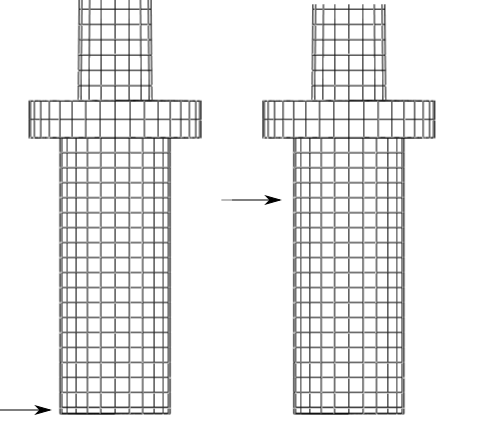
\includegraphics[width=1\textwidth]{figures/load-position.png}
        \caption{Offset from the base of the spigot. Starting at about 1mm on the left.}
    \end{subfigure}
    \caption[Maximum displacement as a function of increasing offset from base of spigot]{Maximum displacement as a function of increasing offset from base of spigot (a), and visualisation of what is meant by increasing the offset from the base of the spigot (b).}
    \label{fig:offset-from-base}
\end{figure}